\documentclass[a4paper, 11pt]{article}
\usepackage{comment} % enables the use of multi-line comments (\ifx \fi)
\usepackage{lipsum} %This package just generates Lorem Ipsum filler text.
\usepackage{fullpage} % changes the margin
\usepackage[utf8]{inputenc}
\usepackage{color}
\usepackage[usenames,dvipsnames]{xcolor}
\usepackage{hyperref} 	%% Use to fix Figure or Table: ex: \begin{table}[H]
\hypersetup{
	%pagebackref=true,
	pdfcreator={LaTeX with abnTeX2},
	pdfkeywords={abnt}{latex}{abntex}{USPSC}{trabalho acadêmico},
	colorlinks=true,       		% false: boxed links; true: colored links
	linkcolor=blue,          	% color of internal links
	citecolor=blue,        		% color of links to bibliography
	filecolor=magenta,      		% color of file links
	urlcolor=blue,
	allbordercolors=black,
	bookmarksdepth=4
}
\usepackage[portuguese]{babel}
\usepackage{graphicx}

\begin{document}
\noindent
\normalsize
 \textbf{Relatório 3, bolsa TT5, processo 2017/14778-4}\\
Processo vinculado: \textbf{2017/05838-3} \\
Coordenadora: \textbf{Dra. Maria Cristina Ferreira de Oliveira} \\
Bolsista: \textbf{Dr. Renato Fabbri}

\section{Informação sobre o nível e período de usufruto da Bolsa}
Este relatório refere-se à bolsa TT5 (Treinamento Técnico nível 5),
vigente inicialmente de 01/Set/2017 até 30/Jun/2019, posteriormente prorrogada até 30/Ago/2019.
O período referente a este relatório é de 31/Jul/2018 até 30/Ago/2019,
de acordo com a prorrogação concedida pela FAPESP.
O bolsista continuou, de 30/Ago/2019, ate hoje, 24/Dez/2019, em atividade eventual, 
por iniciativa própria, principalmente mantendo comunicação com pesquisadores e
mantendo as ferramentas disponibilizadas online.

\section{Atividades realizadas}\label{desc}
As principais contribuições são descritas nas próximas seções.
Busquei
aplicar meus conhecimentos e proficiências nas atividades previstas
no projeto desta bolsa TT5
e no projeto de pesquisa.
Em vista do curto período (2 meses) associado à renovação e ao formato curto
requisitado para este relatório, este documento estende o Relatório 2 já apresentado,
evitando repetir as informações.

\subsection{Visualização interativa de redes bipartidas assistida por estratégias multinível}\label{sml}
Em colaboração com os pesquisadores Alan Valejo, Alneu Andrade, e Cristina Oliveira,
implementei uma nova interface para a navegação das redes em representação multinível
utilizando arestas híbridas. A primeira interface, já apresentada no Relatório 2,
utiliza retângulos translúcidos para representar os vértices sucessores (``super-vértices'')
da rede e manter seus vértices predecessores agrupados, os quais são representados no interior dos retângulos.
Nesta nova interface de navegação, reiterada pelo Alan como intuitiva e talvez ideal como modelo de referência,
quando um vértice sucessor é expandido, os seus vértices predecessores são renderizados no
\emph{canvas} individualmente, sem
evidenciar visualmente o agrupamento no vértice sucessor original,
e as arestas de um vértice são:
i) com vizinho, se o vizinho está explicitamente representado;
ii) com o vértice sucessor do vizinho, se este está explicitamente representado;
iii) com os  predecessores do vizinho, se estes estão explicitamente representados.

As arestas implicadas por (ii) e (iii) são arestas híbridas, i.e. resultado de arestas
de um certo nível e de relações sucessores-predecessores entre dos vértices.
Este modelo implica na necessidade de ajustes no \emph{layout} quando
os vértices são expandidos ou colapsados.
Para possibilitar esta funcionalidade com redes grandes,
esta interface provém também a obtenção do \emph{layout} de rede (i.e. da posições dos vértices)
em tempo real.
A obtenção de \emph{layout}s de redes são de alto custo computacional.
Portanto, foram também exploradas variações de um algoritmo básico potencialmente
mínimo na simplicidade e quantidade de cálculos necessários para a obtenção das posições.
O algoritmo básico foi nomeado ``VICG'', por ter sido criado neste grupo de pesquisa
e por ocasião deste projeto de pesquisa, pelo bolsista.
As variantes disponibilizadas são: \emph{theoretic}, \emph{optimalX}, e \emph{optimalXX}.
A descrição deste algoritmo de \emph{layout} foge ao escopo deste relatório dada a complexidade da descrição necessária.
Em resumo, é um algoritmo iterativo de \emph{layout} baseado em forças cujos cálculos e reposicionamentos dos vértices
são realizados apenas parcialmente em cada iteração e utilizando a distância de Manhattan.
Este algoritmo é potencialmente não descrito na literatura científica e é potencialmente o mais leve possivel,
e o mímino teórico, dentre os `algoritmos iterativos de \emph{layout} baseados em forças'.
Para um uso facilitado por não especialistas, o algoritmos precisa ainda de alguns ajustes,
e a implementação disponibilizada é ainda apenas um protótipo operacional.

Estamos ainda trabalhando em dois incrementos para esta interface: (i)
a reinclusão das \emph{widgets} e funcionalidades responsáveis pela exibição e análise dos histogramas de grau e 
coeficiente de clusterização; (ii) integrar a interface à ferramenta BNOC~\cite{bnoc} para síntese 
de redes bipartidas a partir de parâmetros de entrada definidos pelo usuário.
Assim, espera-se ter uma interface de visualização integrada para o estudo de estratégias
multinível em redes bipartidas. 
Pretendemos também reformular e ressubmeter o artigo citado como submetido no relatório anterior, o qual foi rejeitado.

Para melhorar a qualidade do software, sem prioridade no momento,
concebemos algumas tarefas principais.
São ``issues'' a serem vinculadas ao repositório Git principal:
(i) refatorar e limpar o código para separar as aplicações;
(ii) laço (\emph{loop}) assíncrono para cálculo de posições dos vértices,
atualizando quantas iterações conseguiu realizar,
para auxiliar o usuário a escolher um algoritmo de \emph{layout} de rede;
(iii) usar um \emph{particle system} para vértices e arestas
(testes iniciais indicam que permite a visualização de redes muito maiores;
(iv) uso da GPU para cálculo vetorial (importante para obter \emph{layouts} de redes);
(v) desenvolvimento de uma aplicação mais voltada para ``visual analytics'', considerando os metadados;
(vi) escrever um \emph{script} Bash para colocar no ``cron'' e subir as interfaces sempre que o servidor for reiniciado.

    A nova interface está acessível publicamente em \url{http://rfabbri.vicg.icmc.usp.br:3000/multilevel2/topdown2},
    e um vídeo expositivo em \url{https://youtu.be/VdAVE4AHfi8}.
    A Figura~\ref{ml} exemplifica a interface em uso.

\begin{figure}[h!]
\centering
  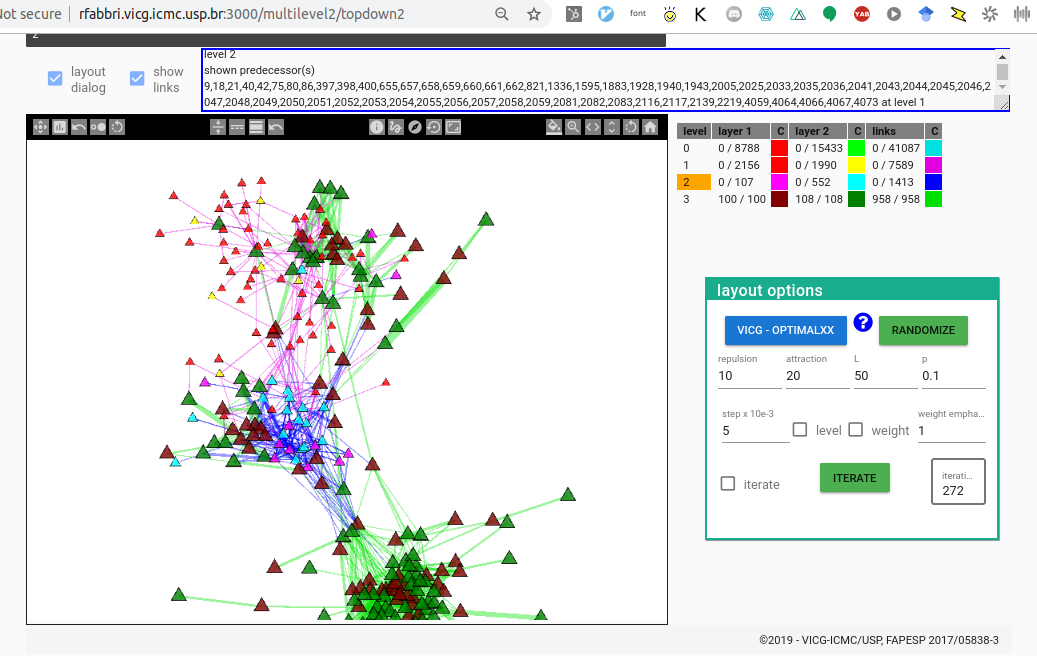
\includegraphics[width=0.8\linewidth]{hybrid}
\caption{%
  Distinto do descrito no relatório anterior, sobre a interface anterior,
  note os vértices de 3 níveis diferentes, relacionados por arestas
  híbridas, sem a utilização de caixas para vértices sucessores expandidos.
  Note também o componente para cálculo das posições dos vértices (i.e. do '\emph{layout} de rede') em tempo real.
}\label{ml}
\end{figure}

\subsection{Visualização interativa de redes utilizando comunicabilidade}\label{scom}
Na continuidade da colaboração com o pesquisador Ernesto Estrada,
pesquisador notório em Redes Complexas, autor de livros e de diversas publicações relevantes para a área~\cite{ern1,ern2,ern3,ern4},
ele apresentou a interface já na ``Latin American Conference on Complex Networks'' (5-9/Ago/2019):
\url{http://rfabbri.vicg.icmc.usp.br:3000/communicability}.
Esta interface passou por diversas versões,
recebeu novos algoritmos de clusterização e de redução de dimensionaldiade,
melhoras no uso das medidas de comunicabilidade, etc.
A Figura~\ref{com} ilustra a forma atual da interface.
Iniciamos a escrita de um artigo sobre a interface e métodos desenvolvidos
e sua utilidade.

\begin{figure}[h!]
\centering
  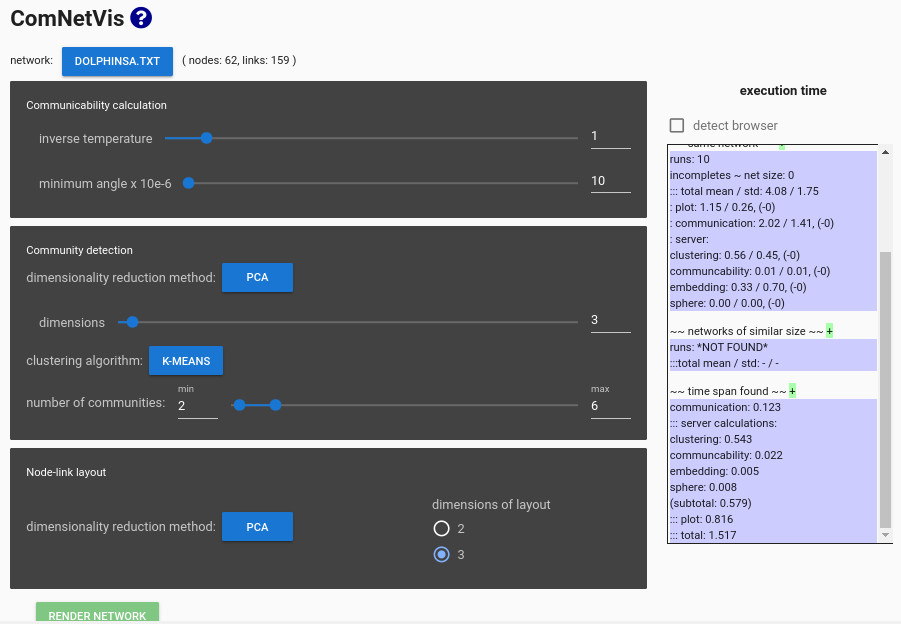
\includegraphics[width=0.8\linewidth]{com}
\caption{%
  Solução final desenvolvida, em colaboração com o pesquisador Estrada.
  Foi fixado o uso dos ângulos de comunicabilidades, e descartado o uso das distâncias.
  Há uma redução de dimensionalidade para a detecção de comunidades,
  outra para a obtenção das posições no plano ou espaço 3D.
  Estão integrados à interface diversos métodos canônicos de clusterização.
  Fez-se também necessária o registro e exibição dos tempos associados às execuções,
  pois alguns dos métodos são custosos em alguns contextos,
  e.g. quando há muitos vértices e/ou arestas.
}\label{com}
\end{figure}


\subsection{Interface para visualização e análise de redes longitudinais}\label{sevo}
Iniciamos a consideração do artigo rejeitado para ressubmissão.
As revisões obtidas na rejeição pareceram positivas quanto às contribuições potencialmente
novas do trabalho. Há, porém, a necessidade de melhor contextualizar e disponibilizar a ferramenta
com facilidades para o uso por uma pessoa não interna à pesquisa.

\subsection{Interface para visualização de redes enriquecidas com texto}
A interface mínima já implementada (\url{https://youtu.be/MH1D8S75d7E}),
continua em consideração e amadurecimento para descrição a aprofundamento
do modelo mínimo de visualização com técnicas de redes complexas, mineração
de texto, e distâncias estatísticas.

\subsection{Visualização para auxílio à análise de paisagens sonoras}\label{pa}
Desenvolvemos uma nova interface de análise de paisagens sonoras com base no
artigo~\cite{eld}.  
Nesta nova versão, um usuário pode adicionar arquivos de áudio ou escolher algum dos disponíveis.
Pode também escolher o número de componentes para a decomposição do som original,
e o código está preparado para adicionar customizações.
As possibilidades de parametrização do método SIPLC2D são muitas, portanto estamos avaliando quais
parametrizações devem ser disponibilizadas na interface.
Além disso, dado que não conseguimos (ainda) decompor o som original nas componentes de um
trecho menor, por enquanto decidimos permitir a análise de um trecho pequeno para escolha da
parametrização a ser aplicada em todo o áudio, pois o método é computacionalmente custoso.
A Figura~\cite{ps} exemplifica a interface em operação.
Esta nova interface está disponível em: \url{http://rfabbri.vicg.icmc.usp.br:3000/soundscape/min},
enquanto a interface inicial foi realocada para: \url{http://rfabbri.vicg.icmc.usp.br:3000/soundscape}.

A Figura~\ref{ss} ilustra a forma atual da interface.

\begin{figure}[h!]
\centering
  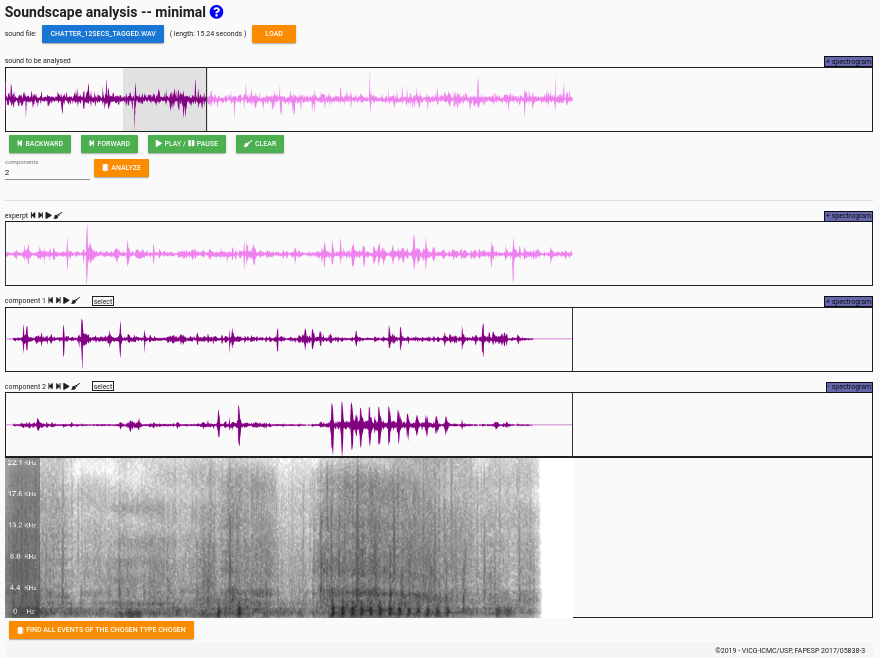
\includegraphics[width=0.8\linewidth]{ss}
\caption{%
  A versão expandida da interface mínima para utilização de SIPLC2D na separação de fontes sonoras.
  Nesta versão, um usuário pode carregar novos arquivos de áudio, escolher o áudio para análise,
  escolher o trecho para análise, o número de componentes, e ouvir individualmente cada componente
  ou o trecho escolhido para análise.
  O usuário também pode observar o espectrograma de qualquer componente, e pode fazer uso de algumas
  funcionalidades para a seleção e audição de trechos de áudio.
}\label{ss}
\end{figure}

\subsection{Disponibilização de dados ligados de redes sociais}
Para dar suporte à pesquisa realizada no VICG, entrei em contato com o
Data.World (apresentado para mim pela profa. Cristina, coordenadora do projeto)
e estabeleci uma colaboração.
Pudemos então disponibilizar publicamente, em RDF, dados das seguintes redes sociais:
Facebook, Twitter, Email, IRC, Participa.br, Cidade Democrática, AA.
Ao todo, estes dados formam redes com centenas de milhares (talvez até alguns milhões)
de participantes, relacionados em geral por amizades, interações, ou critérios de semelhança.
Os dados estão disponíveis em:
\url{https://data.world/rfabbri/linked-open-social-data} (pode ser necessário login na plataforma).
Foi possível também disponibilizar uma biblioteca oficial e simples para o acesso a estes dados,
sem a utilização direta da API do Data.World ou a necessidade de quaisquer credenciais:
\url{https://pypi.org/project/losd/}.
Um artigo com uma descrição sucinta destes dados está disponível em:
\url{https://github.com/ttm/linkedOpenSocialDatabase/raw/master/mdpi/template.pdf},
com arquivo suplementar em:
\url{https://github.com/ttm/linkedOpenSocialDatabase/raw/master/supplementaryDocument.pdf}.


\subsection{Experimentos de visualização para escalar iniciativas sociais}
Em continuidade aos trabalhos reportados em~\cite{tese,virus,sfvideo},
para testar a aplicabilidade das estratégias multiníveis na ``coleta e difusão de informação e bens'',
e na ``propagação de tratos sociais'', iniciei a escrita de software para alcançar interfaces
que permitam ao usuário disparar processos de interação sociais em cadeia, i.e. que envolvem
a propagação de alguma informação (e.g. uma proposta).
Estes testes iniciais foram aproveitados para experimentar sistemas de partículas (recurso WebGL),
medições de duração (para otimização) e projeções planares.
Os códigos desenvolvidos estão todos em JavaScript e são executados no cliente,
com carga mínima para o servidor,
incluindo acesso aos dados ligados, derivação de redes, e obtenção de sequência de redes
em estratégia multinível.
O \emph{framework} utilizado difere dos anteriores, com foco em Meteor.js,
nas bibliotecas Pixi.js (para mapeamentos visuais de dados e elementos visuais interativos),
Tone.js (para mapeamentos sonoros dos dados),
e em requisições HTTP com \emph{queries} SparQL para acesso dos dados da LOSD.
% A Figura~\ref{exp} ilustra minimamente as interfaces desenvolvidas.
% (Preciso de algumas poucas horas adicionais para lidar com estes desenvolvimentos pouco
% finalizados)

\subsection{Parcerias internacionais}
A primeira autora do artigo~\cite{eld}, Alice Eldridge,
manteve contato comigo depois que escrevi para ela sobre
métodos utilizados para as interfaces mencionadas na Seção~\ref{pa}.
Em mensagem de email recente, ela manifestou interesse em
estabelecer uma colaboração acadêmica com nossa pesquisa, e que ``está já
vasculhando as oportunidades para obter verba e formalização da parceria,
no novo contexto de Brexit'' (ela trabalha na Universidade de Sussex).
O Ernesto Estrada manifestou interesse na continuidade do desenvolvimento
das interfaces de visualização de dados para o desenvolvimento e disponibilização
de novas técnicas, acompanhada da publicação de artigos.
Após o período de prorrogação da bolsa, estabeleci colaboração
com empresas, em especial com a BairesDev (Argentina, Vale do Silício/EUA) e
AdRoll/NextRoll/RollWorks (Vale do Silício/EUA). 
Encaminharei estas colaborações para confluir com a continuidade dos
trabalhos realizados neste projeto, e para contato entre os pesquisadores
mais importantes para a minha atuação, a saber com a coordenadora Profa. Cristina,
e com o Dr. Alan Valejo.

\section{Avaliação do impacto das atividades do bolsista sobre o andamento do projeto}
Colaborei no desenvolvimento de métodos, programação de interfaces,
que constarão em artigos submetidos.
Acredito ter auxiliado no andamento do projeto, em conformidade com a bolsa TT5,
e que entre hoje, 24/Dez/2019, e a entrega deste relatório, 30/Jan/2020, acrescentarei
a este relatório avanços na escrita e submissão dos artigos, em conformidade
com o relatório anterior.


\section{Apreciação do desempenho do bolsista (escrita pela coordenadora)}
% para Cristina escrever
( copiado do relatório anterior )

O bolsista tem grande conhecimento em métodos na área de redes complexas e em
programação. Assim, tem contribuído significativamente no desenvolvimento de
ferramentas que mostram-se fundamentais como provas-de-conceito de diversas
técnicas investigadas no âmbito do projeto. Ele tem interagido mais
intensamente com os pesquisadores que atuam na frente de pesquisa em métodos
multinível em redes complexas, com potencial para interagir também com
pesquisadores que atuam na frente de pesquisa em paisagens acústicas. Acredito
também que o projeto apresentou a ele uma nova gama de conhecimentos em
visualização de dados, abrindo novas perspectivas para a sua atuação futura
como pesquisador. Minha avaliação é que o bolsista está contribuindo de maneira
relevante para ampliar os resultados gerados no âmbito do projeto de pesquisa.

\bibliographystyle{unsrt}
\bibliography{pbib}

\end{document}

